\documentclass[12pt,a4paper,oneside,english,brazil]{abntex2}
\usepackage[utf8]{inputenc}
\usepackage{graphicx}
\usepackage[alf]{abntex2cite}
\titulo{Importação de Documentos Acadêmicos}
\autor{Maria Oliveira}
\local{Recife}
\data{2025}
\orientador{Prof. Dr. João Santos}
\instituicao{Universidade Federal de Pernambuco \par Centro de Informática}
\tipotrabalho{Trabalho de Conclusão de Curso}
\preambulo{Monografia apresentada ao curso de Ciência da Computação.}
\newcommand{\sigla}[1]{\textsc{#1}}
\begin{document}
\imprimircapa
\imprimirfolhaderosto
\begin{resumo}
Este trabalho apresenta um conversor de documentos.

\textbf{Palavras-chave}: Pandoc. Typst. ABNT.
\end{resumo}
\begin{resumo}[Abstract]
\begin{otherlanguage*}{english}
This work presents a document converter.

\vspace{\onelineskip}
\noindent
\textbf{Keywords}: Pandoc. Typst.
\end{otherlanguage*}
\end{resumo}
\tableofcontents*
\textual
\chapter{Introdução}
O formato \sigla{ABNT} é exigido \cite[p.~42]{silva2020}. Segundo \citeonline{souza2019}, a tipografia importa\footnote{Ver também o manual do Typst.}.

A equação de Einstein $E = mc^2$ é famosa, assim como:
\begin{equation}
\int_0^1 x^2 \, dx = \frac{1}{3}
\end{equation}

\begin{citacao}
A tipografia é a arte de dispor o texto de forma legível e agradável, servindo ao leitor antes de tudo \cite[p.~10]{souza2019}.
\end{citacao}

\section{Objetivos}
\begin{itemize}
  \item Converter arquivos \textit{LaTeX};
  \item Preservar \textbf{citações}.
\end{itemize}

\chapter{Metodologia}
\begin{figure}[h]
  \centering
  \caption{Arquitetura do sistema}
  \label{fig:arq}
  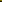
\includegraphics[width=0.8\textwidth]{figuras/arquitetura}
  \legend{Fonte: Elaborado pelo autor (2025).}
\end{figure}

\begin{table}[h]
\caption{Resultados obtidos}
\begin{tabular}{lc}
\hline
Formato & Acurácia \\
\hline
DOCX & 95\% \\
LaTeX & 90\% \\
\hline
\end{tabular}
\fonte{Dados da pesquisa.}
\end{table}

\section*{Considerações}
Texto final.

\bibliography{referencias}
\end{document}
